\documentclass[12pt]{report}

% Pour le bon support de la langue française : 
\pdfminorversion=5
\pdfobjcompresslevel=2
\usepackage[T1]{fontenc}
\usepackage[utf8]{inputenc}
\usepackage{lmodern}

\usepackage{etex}
\usepackage{lipsum}

% Packages perso :
\usepackage{soul}
\usepackage{fancyhdr}
\usepackage{boxedminipage}
\usepackage{makeidx}
\makeindex
\usepackage{caption}
\usepackage[final]{pdfpages}
\usepackage{listings} % pour inclure des algorithmes
\newcommand{\deriv}{\mathrm{d}}

\usepackage{color} % définit une nouvelle couleur
\usepackage{xcolor}             % Pour mettre de la couleur
% Bibliographie dans la Table des matières
%\usepackage[nottoc, notlof, notlot]{tocbibind} 
\usepackage{authoraftertitle}   %\MyAuthor

\usepackage{float}              % Pour les figures
\usepackage{pgfplots}
\usepackage{tikz}
\usetikzlibrary{arrows,shapes,positioning}
\usetikzlibrary{decorations.markings,decorations.pathmorphing,
decorations.pathreplacing}
\usetikzlibrary{calc,patterns,shapes.geometric}
\tikzset{every picture/.style={execute at begin picture={
\shorthandoff{:;!?};}
}}
\usepackage[europeancurrents,europeanresistors,cuteinductors,europeanports,europeanvoltages]{circuitikz}         % Circuits électriques
\usepackage{thumbpdf}           % Fichier pdf généré 
                                % contien une              
                                % miniature de chaque slide 
%\usepackage{frbib}              % Bibliographie en fr
\usepackage{dashrule}           % Lignes points-tillés
\usepackage{pifont}             % \ding{code utf8}
\usepackage{hyperref}           % Pour ajouter des liens avec \href
\usepackage{lastpage}           % Avoir total de pages dans le footer.
\usepackage{graphicx}           % Pour les images et figures
\usepackage{wrapfig}            % Pour détourer les figures
%\begin{wrapfigure}[lineheight]{alignement}{width}
\usepackage{multicol}           % Doc sur plusieurs colonnes
\setlength{\columnseprule}{.4pt}% Avec séparateur.
\usepackage{fancybox}           % De chouettes encadrements
\usepackage{lettrine}           % Pour de beaux paragraphes
% \usepackage{type1cm}          % scalable fonts pour lettrine
\usepackage{oldgerm}            % Lettrines en gothique
\newcommand{\gothique}[2]{\lettrine{\textgoth #1}{#2}} 
\usepackage{yfonts}             % De belles enluminures
\newcommand{\enluminure}[2]{\lettrine[lines=3]{\small \initfamily #1}{#2}} 
\usepackage{url}                % Pour écrire des url
\usepackage{geometry}
\geometry{margin=60pt}
\usepackage{setspace}           % Pour changer l'interligne
\usepackage{eurosym}            % Pour le signe \euro
\usepackage{colortbl}           % Couleur dans tableaux
\usepackage{tabularx}           % pour des tableaux à taille de la page
\usepackage{longtable}          % Pour les grands tableaux
\usepackage[tight]{shorttoc}    % Pour faire un sommaire à la française.
\newcommand{\sommaire}{\shorttoc{Sommaire}{1}}
\usepackage{array}              % De beaux tableaux
\usepackage{multirow}           % Tableaux sur plusieurs lignes
                                % \multirow{nlignes}{largeur ou *}{contenu}
\usepackage{amsmath}            % Un peu de maths
\usepackage{amssymb}            % Encore des maths
\usepackage{mathtools}
\usepackage{empheq}             % Pour encadrer les équations
\usepackage{pdfpages}           % Pour include des pdf avec
%\includepdf[pages=-]{votre_fichier} 
% ,pagecommand={}               % Pour aussi mettre le num de la page
\usepackage[normalem]{ulem}               % Pour barrer du texte

\usepackage{pgfpages}           % Pour avoir 2 pages sur A4 paysage
\usepackage{datetime}           % Jouer facilement avec les dates
% Pour la physique : 
\usepackage{numprint}           % Pour faire des groupes de 3 nombres
\usepackage[squaren,Gray,cdot]{SIunits} % Unités SI
% Ecrire des symboles atomiques
\newcommand{\noyau}[3]{\prescript{#2}{#3}{\mathrm{#1}}}
% Utilisation $\noyau{C}{12}{6}$

% Pour la chimie : 
\usepackage[version=3]{mhchem}
\usepackage{chemfig}

%%%
% Commandes

% Ajout d'une image avec label
\newcommand{\image}[3]{
% \image{fichier}{label}{description}
\begin{center}
% Nécessite le package float
\begin{figure}[H]
\includegraphics[width=0.8\textwidth]{#1}
\caption{\label{#2}{#3}}
\end{figure}
\end{center}
}

% Ajout d'une image largeur page avec label
\newcommand{\imagebig}[3]{
% \imagebig{fichier}{label}{description}
\begin{center}
% Nécessite le package float
\begin{figure}[H]
\includegraphics[width=1\textwidth]{#1}
\caption{\label{#2}{#3}}
\end{figure}
\end{center}
}

% Une image qui prend toute la page
\newcommand{\imagefull}[1]{
    \newgeometry{margin=0cm}
\begin{center}
\begin{figure}[H]
\includegraphics[width=0.96\paperwidth]{#1}
\end{figure}
\end{center}
\restoregeometry
\nopagebreak
}

% Un encadré grisé
\newcommand{\encadregris}[1]{
\begin{center}
\colorbox{gray!20}{
\begin{minipage}{0.95\textwidth}
{#1}
\end{minipage}
}
\end{center}
}

% Un mot grisé
\newcommand{\motgris}[1]{
\colorbox{gray!20}{{#1}}
}

% Un encadré
\newcommand{\encadre}[1]{
\begin{center}
\fbox{
\begin{minipage}{0.95\textwidth}
{#1}
\end{minipage}
}
\end{center}
}

% flèche
\newcommand{\ra}[0]{
    $\rightarrow$
}

% Image détourée
% \wrapimg{align}{width}{img}
\newcommand{\wrapimg}[3]{
\begin{wrapfigure}{#1}{#2}
\includegraphics[width={#2}]{#3}
\end{wrapfigure}
}

\newcommand{\hdr}[0]{
    \hdashrule{1cm}{1pt}{1pt}
}

\newcommand{\hdrp}[0]{
    \hdashrule{3cm}{1pt}{1pt}
}

\newcommand{\hdrpp}[0]{
    \hdashrule{4cm}{1pt}{1pt}
}

\newcommand*{\etoile}
{
\begin{center}
*\par
*\hspace*{3ex}*
\end{center}
}

% petit carré
\newcommand{\petitcarre}{\rule[.2ex]{0.75ex}{0.75ex}}

%incertitude relative
\newcommand{\incertRel}[1]{
    \frac{\Delta {#1}}{{#1}}
}

% listes avec puces carrées
\newcommand{\carlst}[1]{
    \begin{itemize}
    \renewcommand\labelitemi{\petitcarre}
    {#1}
    \end{itemize}
}

% \emph plus simple
\newcommand{\e}[1]{\emph{{#1}}}

% equation encadrée
\newcommand{\boxeq}[1]{
    \begin{empheq}[box=\shadowbox]{align}
    {#1}
    \end{empheq}
}

%%% Schémas de chimie %%%

% Schema de titrage
% \schemaTitrage{solution titrante}{solution titrée}
\newcommand{\schemaTitrage}[2]{
    \begin{tikzpicture}
        \draw [thick]
        (0,0) -- ++ (2,0) -- ++ (0,1) -- ++ (-2,0) -- ++ (0,-1)
        (0.3,3) -- ++ (0,-2)
        (1.7,3) -- ++ (0,-2)
        (1,6) -- ++ (0,-3)
        (0.8,3.3) -- ++ (0.4,0)
        (0.3,1.7) -- ++ (1.4,0)
        (0.3,0.3) circle(0.1)
        (1,1.11)ellipse (0.25 and 0.10) 
        ;
        \draw
        [<-,>=stealth] (1,4.4) -- ++ (1.5,0) node[right]  {
            \begin{minipage}{0.275\textwidth}
                {#1}
            \end{minipage}
        }
        ;
        \draw
        [<-,>=stealth] (1,1.5) -- ++ (1.5,0) node[right] {
            \begin{minipage}{0.27\textwidth} 
            {#2}
            \end{minipage}
        }
        ;
    \end{tikzpicture}
}

% Tube à essai légendé.
\newcommand{\schemaTubeEssai}[1]{
    \begin{tikzpicture}[scale=0.25]
    \draw
    (0,0) arc (0:-180:1)
    (-2,0) -- ++ (0,8)
    (0,0) -- ++ (0,8)
    (-2,4) -- ++ (2,0)
    (-0.5,-1) node[below] 
        {
        \begin{minipage}{0.2\textwidth}
        {#1}
        \end{minipage}
        }
    ;
    \end{tikzpicture}
}
% Papier millimétré
% \papmili{x}{y}
\newcommand{\papmili}[2]{
\begin{tikzpicture}
\draw[step=1mm, line width=0.1mm, black!30!white] (0,0) grid
({#1},{#2});
\draw[step=5mm, line width=0.2mm, black!40!white] (0,0) grid
({#1},{#2});
\draw[step=5cm, line width=0.5mm, black!50!white] (0,0) grid
({#1},{#2});
\draw[step=1cm, line width=0.3mm, black!90!white] (0,0) grid
({#1},{#2});
\end{tikzpicture}
}
% \grap{x}{y}{legende x}{legende y}
\newcommand{\graph}[4]{
\begin{tikzpicture}
\draw[step=1mm, line width=0.1mm, black!30!white] (0,0) grid
({#1},{#2});
\draw[step=5mm, line width=0.2mm, black!60!white] (0,0) grid
({#1},{#2});
\draw[step=5cm, line width=0.5mm, black!80!white] (0,0) grid
({#1},{#2});
\draw[line width=0.6mm, ->, >=stealth] (0,0) -- ({#1},0)
node[right]{{#3}};
\draw[line width=0.6mm, ->, >=stealth] (0,0) -- (0,{#2})
node[above]{{#4}};
\end{tikzpicture}
}

\usepackage{listingsutf8}

\lstdefinestyle{customc}{
  belowcaptionskip=1\baselineskip,
  breaklines=true,
  frame=L,
  xleftmargin=\parindent,
  language=C,
  showstringspaces=false,
  basicstyle=\footnotesize\ttfamily,
  keywordstyle=\bfseries\color{green!40!black},
  commentstyle=\itshape\color{purple!40!black},
  identifierstyle=\color{blue},
  stringstyle=\color{orange},
}

\lstdefinestyle{customasm}{
  belowcaptionskip=1\baselineskip,
  frame=L,
  xleftmargin=\parindent,
  language=[x86masm]Assembler,
  basicstyle=\footnotesize\ttfamily,
  commentstyle=\itshape\color{purple!40!black},
}

\lstset{escapechar=@,style=customc}

\pagestyle{fancy}
\fancyhead[L]{}
\fancyhead[R]{}
\fancyfoot[L]{}
\fancyfoot[R]{}


\begin{document}

\newlength{\larg}
\setlength{\larg}{14.5cm}
\lstset{inputencoding=utf8/latin1}
\title{
{\rule{\larg}{1mm}}\vspace{7mm}
\begin{tabular}{p{0cm} c}
   & { {\textbf{Tutorial}}} \\
   & {\huge Lighting and shadow mapping} \\
\end{tabular}\\
\vspace{2mm}
{\rule{\larg}{1mm}}
\vspace{2mm} \\
\begin{tabular}{p{11cm} r}
   & {\large  25/08/2016}
\end{tabular}\\
\vspace{2cm}
\large{\textit{} \\
BANGOR UNIVERSITY\\
School of Computer Science}
\vspace{5cm}
}
\author{\begin{tabular}{p{13.7cm} r}
Andréas MEULEMAN
\end{tabular}\\
\hline }
\date{}
\maketitle

\chapter{Introduction}

	The complete source code of this tutorial is available on the Subversion (SVN) repository at $tutorials/tutorial\_05\_qt4$. 
	
	$DepthMap$ is a class to handle and generate a depth map of a set of polygon mesh using a framebuffer. We are going to use this class to create a shadow map and the shaders $display\_realistic\_gl3.vert$ and $display\_realistic\_gl3.frag$ will enable us to get lightings easely.
	
\chapter{includes}

These are to use the shaders $display\_realistic\_gl3.vert$ and $display\_realistic\_gl3.frag$:
\begin{lstlisting}
#include "display_realistic_gl3.frag.h"
#include "display_realistic_gl3.vert.h"

#ifndef GVXR_MATRIX4X4_H
#include "gVirtualXRay/Matrix4x4.h"
#endif

#ifndef GVXR_SHADER_H
#include "gVirtualXRay/Shader.h"
#endif
\end{lstlisting}

We have to include the header of the class we are going to use:
\begin{lstlisting}
#include "gVirtualXRay/DepthMap.h"
\end{lstlisting}

\chapter{Add lighting}

\subsection{Initialize variables}

The display shader requires a light direction for lighting, we have to initialize it before the rendering:

\begin{lstlisting}
	m_light_direction = VEC3(-1, 3, -0.5);
	m_light_direction.normalize();
\end{lstlisting}

we also have to initialize the light colours:

\begin{lstlisting}
 	// Define the light colours here
   	GLfloat light_global_ambient[] = { 0.2, 0.2, 0.2, 1.0 };
   	GLfloat light_ambient[] = { 0.2, 0.2, 0.2, 1.0 };
   	GLfloat light_diffuse[] = { 1.0, 1.0, 1.0, 1.0 };
   	GLfloat light_specular[] = { 1.0, 1.0, 1.0, 1.0 };
\end{lstlisting}

\subsection{Define uniforms inputs for the display shader}

To make the display shader use lighting: 

\begin{lstlisting}
        // Handle for shader variables
    	GLuint handle(0);

        //use lighting
        GLint lighting;
        lighting = 1;
        handle = glGetUniformLocation(shader_id,"g_use_lighting");
        glUniform1iv(handle, 1, &lighting);
        checkOpenGLErrorStatus(__FILE__, __FUNCTION__, __LINE__);
\end{lstlisting}

The light direction and colours:

\begin{lstlisting}
        handle = glGetUniformLocation(shader_id, "light_global_ambient");
        glUniform4fv(handle, 1, &light_global_ambient[0]);
        checkOpenGLErrorStatus(__FILE__, __FUNCTION__, __LINE__);

        handle = glGetUniformLocation(shader_id, "light_ambient");
        glUniform4fv(handle, 1, &light_ambient[0]);
        checkOpenGLErrorStatus(__FILE__, __FUNCTION__, __LINE__);

        handle = glGetUniformLocation(shader_id, "light_diffuse");
        glUniform4fv(handle, 1, &light_diffuse[0]);
        checkOpenGLErrorStatus(__FILE__, __FUNCTION__, __LINE__);

        handle = glGetUniformLocation(shader_id, "light_specular");
        glUniform4fv(handle, 1, &light_specular[0]);
        checkOpenGLErrorStatus(__FILE__, __FUNCTION__, __LINE__);

        handle = glGetUniformLocation(shader_id, "light_direction");
        glUniform3f(handle, m_light_direction.getX(), m_light_direction.getY(), m_light_direction.getZ());
        checkOpenGLErrorStatus(__FILE__, __FUNCTION__, __LINE__);
\end{lstlisting}

Set the projection and the model matrix: 
\begin{lstlisting}
    	handle = glGetUniformLocation(shader_id, "g_projection_matrix");
        glUniformMatrix4fv(handle, 1, GL_FALSE, g_current_projection_matrix.get());
        checkOpenGLErrorStatus(__FILE__, __FUNCTION__, __LINE__);

        handle = glGetUniformLocation(shader_id, "g_modelview_matrix");
        glUniformMatrix4fv(handle, 1, GL_FALSE, g_current_modelview_matrix.get());
        checkOpenGLErrorStatus(__FILE__, __FUNCTION__, __LINE__);
\end{lstlisting}

In case we want the light direction to be fixed to the camera, we have to send the model matrix for the normal vectors:
\begin{lstlisting}
        MATRIX4 normal_matrix(g_current_modelview_matrix);
        handle = glGetUniformLocation(shader_id, "g_normal_matrix");
        glUniformMatrix3fv(handle, 1, GL_FALSE, normal_matrix.get3x3());
        checkOpenGLErrorStatus(__FILE__, __FUNCTION__, __LINE__);
\end{lstlisting}


\chapter{Add shadows}

\subsection{Build the object}

	the constructor of $DepthMap$ has a parameters of type $unsigned$ $int$: $texture\_size$. It represent the size in pixels of the side of the texture used for the depht map. Its default value is 8192 but it can be modified depending on the graphic card's amount of vram.
	
\subsection{Build the shadow map matrix}

We build the shadow map projection matrix for an orthogonal projection of everything within the coordinates $[-10, 10]$ of all the axis: 

\begin{lstlisting}
    	gVirtualXRay::Matrix4x4<GLfloat> shadowProjectionMatrix(gVirtualXRay::buildOrthoProjectionMatrix(-10.f, 10.f, -10.f, 10.f, -10.f, 10.f));
\end{lstlisting}

The we create the shadow map view matrix using the light direction:
\begin{lstlisting}
    	gVirtualXRay::Matrix4x4<GLfloat> shadowViewMatrix(gVirtualXRay::buildLookAtModelViewMatrix(
    			m_light_direction,
    			gVirtualXRay::VEC3(0.f, 0.f, 0.f),
    			gVirtualXRay::VEC3(0.f, 1.f, 0.f)
    		));
\end{lstlisting}

We multiply the shadow view matrix by the scene model matrix:

\begin{lstlisting}
    	shadowViewMatrix *= m_scene_rotation_matrix;
\end{lstlisting}

\subsection{Render to the shadow map}

First, we create the vector of polygon meshes containing all the meshes that will cast shadows on other objects:

\begin{lstlisting}
    	std::vector<PolygonMesh*> polygon_mesh_set;
    	polygon_mesh_set.push_back(&m_blue_cube_mesh);
    	polygon_mesh_set.push_back(&m_red_cube_mesh);
\end{lstlisting}

\subsubsection{In case all the polygon meshes share the same model matrix}

We multiply the shadow model view matrix by the models projection matrix:

\begin{lstlisting}
    	shadowViewMatrix *= m_meshes_model_matrix;
\end{lstlisting}

We create the shadow MVP matrix by multiplying the projection and the model view matrix:

\begin{lstlisting}
    	gVirtualXRay::Matrix4x4<GLfloat> shadow_matrix=shadowProjectionMatrix*shadowViewMatrix;
\end{lstlisting}

We use the overload of the $render$ function that doesn't use a different matrix per polygon mesh:

\begin{lstlisting}
    	//render to the shadow map
        m_shadow_map.render(polygon_mesh_set, shadow_matrix);
\end{lstlisting}

\subsubsection{In case the polygon meshes have different model matrix}

We don't multiply the shadow matrix by the model projection matrix and we build the vector of matrixes:

\begin{lstlisting}
	std::vector<Matrix4x4<float > > matrix_set;
	matrix_set.push_back(m_blue_cube_model_matrix);
	matrix_set.push_back(m_red_cube_model_matrix);
\end{lstlisting}

We use the overload of $render$ that uses a different matrix per polygon mesh:

\begin{lstlisting}
    	//render to the shadow map
        m_shadow_map.render(polygon_mesh_set, shadow_matrix, matrix_set);
\end{lstlisting}

In that case, we obviously need to change the model view matrix and the normal matrix for all the polygon meshes before defining the display shader inputs.

\subsection{use the shadow map}

We have to send the shadow matrix to the display shader:

\begin{lstlisting}
        handle = glGetUniformLocation(shader_id, "g_shadow_map_matrix");
        glUniformMatrix4fv(handle, 1, GL_FALSE, shadow_matrix.get());
        gVirtualXRay::checkOpenGLErrorStatus(__FILE__, __FUNCTION__, __LINE__);
\end{lstlisting}

and the shadow map texture:

\begin{lstlisting}
        //Bind the shadow map texture in texture unit 0
        glActiveTexture(GL_TEXTURE0);
        glBindTexture(GL_TEXTURE_2D, m_shadow_map.getMapTexture());

        handle = glGetUniformLocation(shader_id, "g_shadow_map");
        glUniform1i(handle,0);
        checkOpenGLErrorStatus(__FILE__, __FUNCTION__, __LINE__);
\end{lstlisting}

\chapter{Display the polygon meshes using OpenGL}

Now we just have to define the shader's inputs of the polygon meshes to be rendered and to display them:

\begin{lstlisting}
	    // Get the material
	    Material& material(m_blue_cube_mesh->getMaterial());

	    // Define colours inshader
	    GLuint handle(glGetUniformLocation(aShaderID, "material_ambient"));
	    glUniform4fv(handle, 1, &(material.getAmbientColour()[0]));
	    checkOpenGLErrorStatus(__FILE__, __FUNCTION__, __LINE__);

	    handle = glGetUniformLocation(aShaderID, "material_diffuse");
	    glUniform4fv(handle, 1, &(material.getDiffuseColour()[0]));
	    checkOpenGLErrorStatus(__FILE__, __FUNCTION__, __LINE__);

	    handle = glGetUniformLocation(aShaderID, "material_specular");
	    glUniform4fv(handle, 1, &(material.getSpecularColour()[0]));
	    checkOpenGLErrorStatus(__FILE__, __FUNCTION__, __LINE__);

	    handle = glGetUniformLocation(aShaderID, "material_shininess");
	    glUniform1f(handle, material.getShininess());
	    checkOpenGLErrorStatus(__FILE__, __FUNCTION__, __LINE__);
	    
	    m_blue_cube_mesh.display;
\end{lstlisting}

This must be done for all the meshes.

\chapter{result}

A shadow is cast from the blue cube to the red one:\\

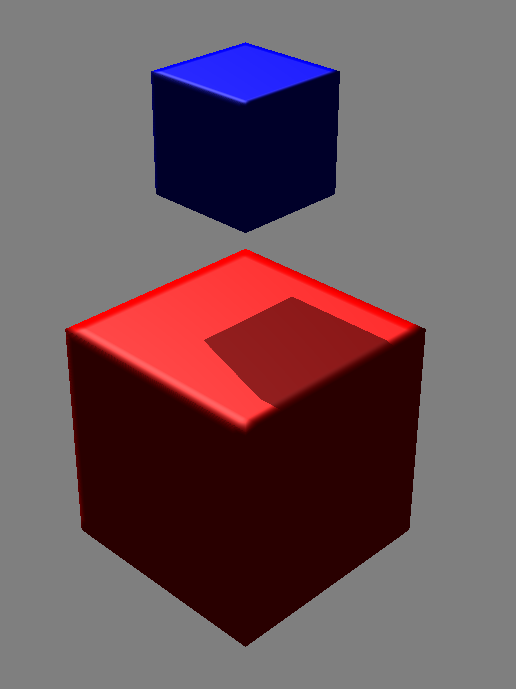
\includegraphics[scale = 0.6]{img/cubes.png}


\newpage
We can combine lighting with the classes inheriting from AnatomicalMesh to get a better rendering:

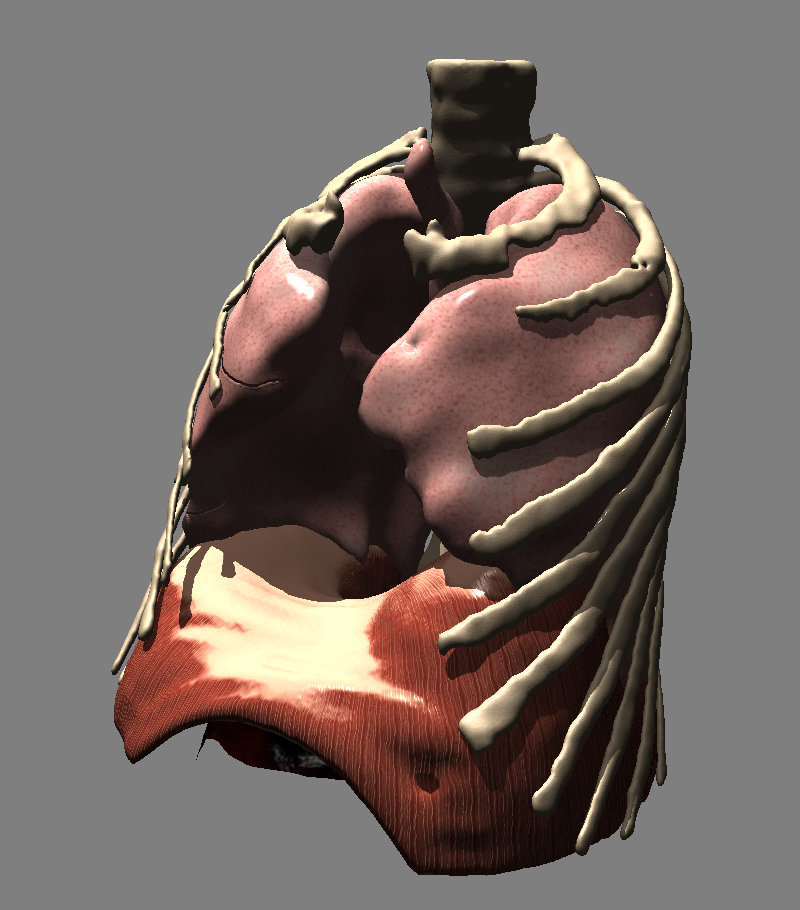
\includegraphics[scale = 0.6]{img/AllMeshesLighting.png}
 
\end{document}